La Business Intelligence (BI) indica l'operazione di inferenza di informazioni da una mole di dati, provenienti da fonti differenti nei processi aziendali. 

In senso ampio, le fonti di informazioni utili possono essere tra le pi� disparate, da statistiche di utilizzo dei sistemi informativi, ai dati generati dal funzionamento di software di automazione, al campionamento di flussi di navigazione e modalit� di utilizzo dei sistemi.

L'obiettivo della BI � di trarre informazioni e conclusioni utili ai fini aziendali, come l'individuazione delle cause di problemi, la misurazione delle performance, la progettazione di \textit{feature} che potrebbero incrementare la qualit� del prodotto o fare previsioni e stime di scenari futuri, sulla base della storia pregressa.

Poich\'{e} i log sono strettamente legati al funzionamento delle applicazioni stesse, possono essere utilizzati, oltre che come sistema di controllo dei malfunzionamenti anche come veicolo di raccolta di informazioni utili alla BI.

La BI, infatti, si avvale dei log con diversi fini:
\begin{itemize}
\item come strumento per la comprensione e il tracciamento del comportamento degli utenti che operano nel sistema
\item per ottenere statistiche di utilizzo del sistema, come ad esempio le funzionalit� pi� utilizzate di un'applicazione o quali aree pi� visitate di un sito internet. 
\end{itemize}

Poich\'{e} i dati utili da collezionare variano in maniera significativa da applicazione ad applicazione, da contesto a contesto, l'idea di costruire un sistema di centralizzazione dei log, che non ponga vincoli nella formulazione degli stessi, va nell'ottica di poter offrire uno strumento utile di raccolta di informazioni diversificate a supporto alle decisioni.

In altre parole, il sistema pu� diventare un collettore di informazioni relative al funzionamento del sistema ma non necessariamente legate ai concetti di errore e criticit�, divenendo di fatto uno strumento per la gestione strategica dei processi aziendali. Un esempio di tool adatto a questo tipo di elaborazioni � SpagoBI \cite{website:SpagoBI}.

\subsubsection{SpagoBI}

SpagoBI � una \textit{suite} open-source ideata appositamente per la Business Intelligence. Questo strumento offre molte funzionalit� per l'elaborazione dei dati e possiede una serie di tool per l'analisi semantica. La fruizione dei dati da parte degli utenti � molto efficace, SpagoBI offre infatti \textit{widget} grafici per la visualizzazione di dati aggregati e complessi, come grafici e riferimenti geospaziali.

\begin{figure}[h]
\centering
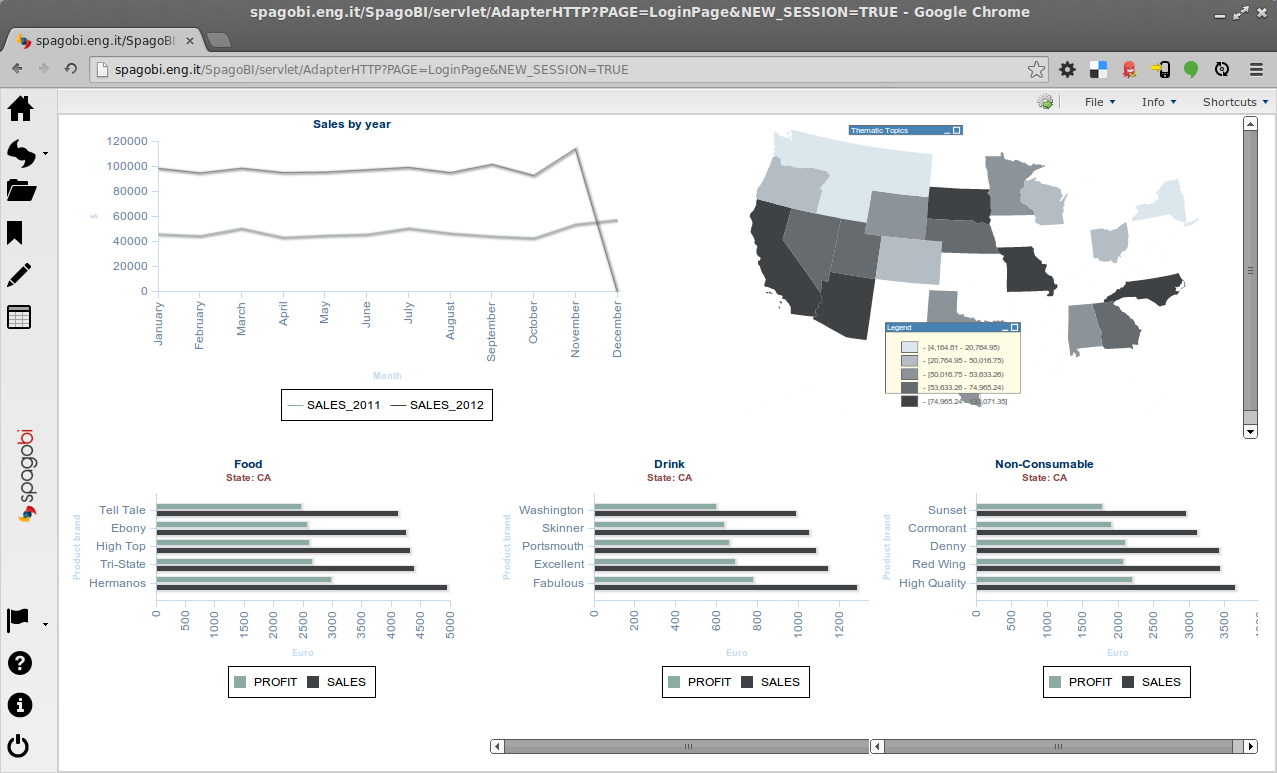
\includegraphics[width=0.7\linewidth]{./img/spagobi}
\caption[Esempio di applicazione realizzata con SpagoBI]{Esempio di applicazione realizzata con SpagoBI}
\label{fig:spagobi}
\end{figure}

SpagoBI possiede una architettura modulare, nella quale ogni componente software possiede un compito specifico e coopera con le altre per realizzare funzionalit� complesse.

\begin{description}
\item[SpagoBI Server] il modulo principale. Il suo compito � offrire le funzionalit� di base per la raccolta, l'analisi e il filtraggio dei dati.
\item[SpagoBI Studio] fornisce agli sviluppatori la possibilit� di modificare i \textit{report} generati da SpagoBI Server secondo le necessit� applicative specifiche.
\item[SpagoBI Meta] offre funzionalit� di elaborazione dei \textit{meta-dati} gestiti dall'applicazione.
\item[SpagoBI SDK] � un tool per l'integrazione di funzionalit� specifiche realizzate da terze parti, ad esempio servizi web o portali esterni all'applicazione.
\end{description}